\chapter{Firmware inerciální jednotky}
Firmware hlavního \ac{MCU} byl vyvíjen pomocí volně dostupného \ac{IDE} poskytovaného výrobcem - \emph{STM32CubeIDE}. Jedná se o nástroj určený pro práci s jazyky C/C++, GCC kompilátorem založeném na Eclipse \cite{V2Tf5wsrbWcbQdoW}. Zároveň poskytuje grafické rozhraní pro konfiguraci a generování knihoven založených na \ac{HAL}, možnost použití \ac{RTOS} a ladící prostředí.

V této práci byly použity poskytované knihovny HAL a FreeRTOS pro ulehčení a urychlení vývoje firmwaru. Jejich použití často s sebou nese nevýhody, jako je například horší využití paměti, nebo výpočetního výkonu, z tohoto důvodu byl zvolen takový \ac{MCU}, aby měl dostatečné rezervy pro jejich použití.
\section{HAL}
Generování kódu \ac{HAL} v  STM32CubeIDE je možné pomocí grafického rozhraní, které poskytuje uživateli možnost nastavení jednotlivých pinů, periferií, komunikačních rozhraní a vnitřních hodin (obrázek \ref{fig:cubeConfig}). Vygenerované knihovny následně umožňují uživateli pracovat s \ac{MCU} s jistou mírou abstrakce, například není nutné znát a pracovat s názvy jednotlivých registrů. Typickým příkladem můžou být komunikační sběrnice (\ac{SPI}, \ac{I2C} \ldots), pro které jsou dostupné obslužné funkce na čtení a vysílání dat, jak v blokujícím režimu, tak i v neblokujícím (například pomocí \ac{DMA}). \cite{V2Tf5wsrbWcbQdoW}

Dále je možné pomocí stejného grafického rozhraní importovat rozšiřující softwarové balíčky, i když už se nejedná přímo o \ac{HAL}. V této práci byly použity \emph{FATFS} pro manipulaci se soubory na microSD kartě, \emph{FreeRTOS} jakožto jeden z dostupných \ac{RTOS} a \emph{USB\_DEVICE} pro práci s \ac{USB} rozhraním třídy \ac{MSC}.

\begin{figure}[h]
     \centering
     \begin{subfigure}[b]{0.4\textwidth}
         \centering
         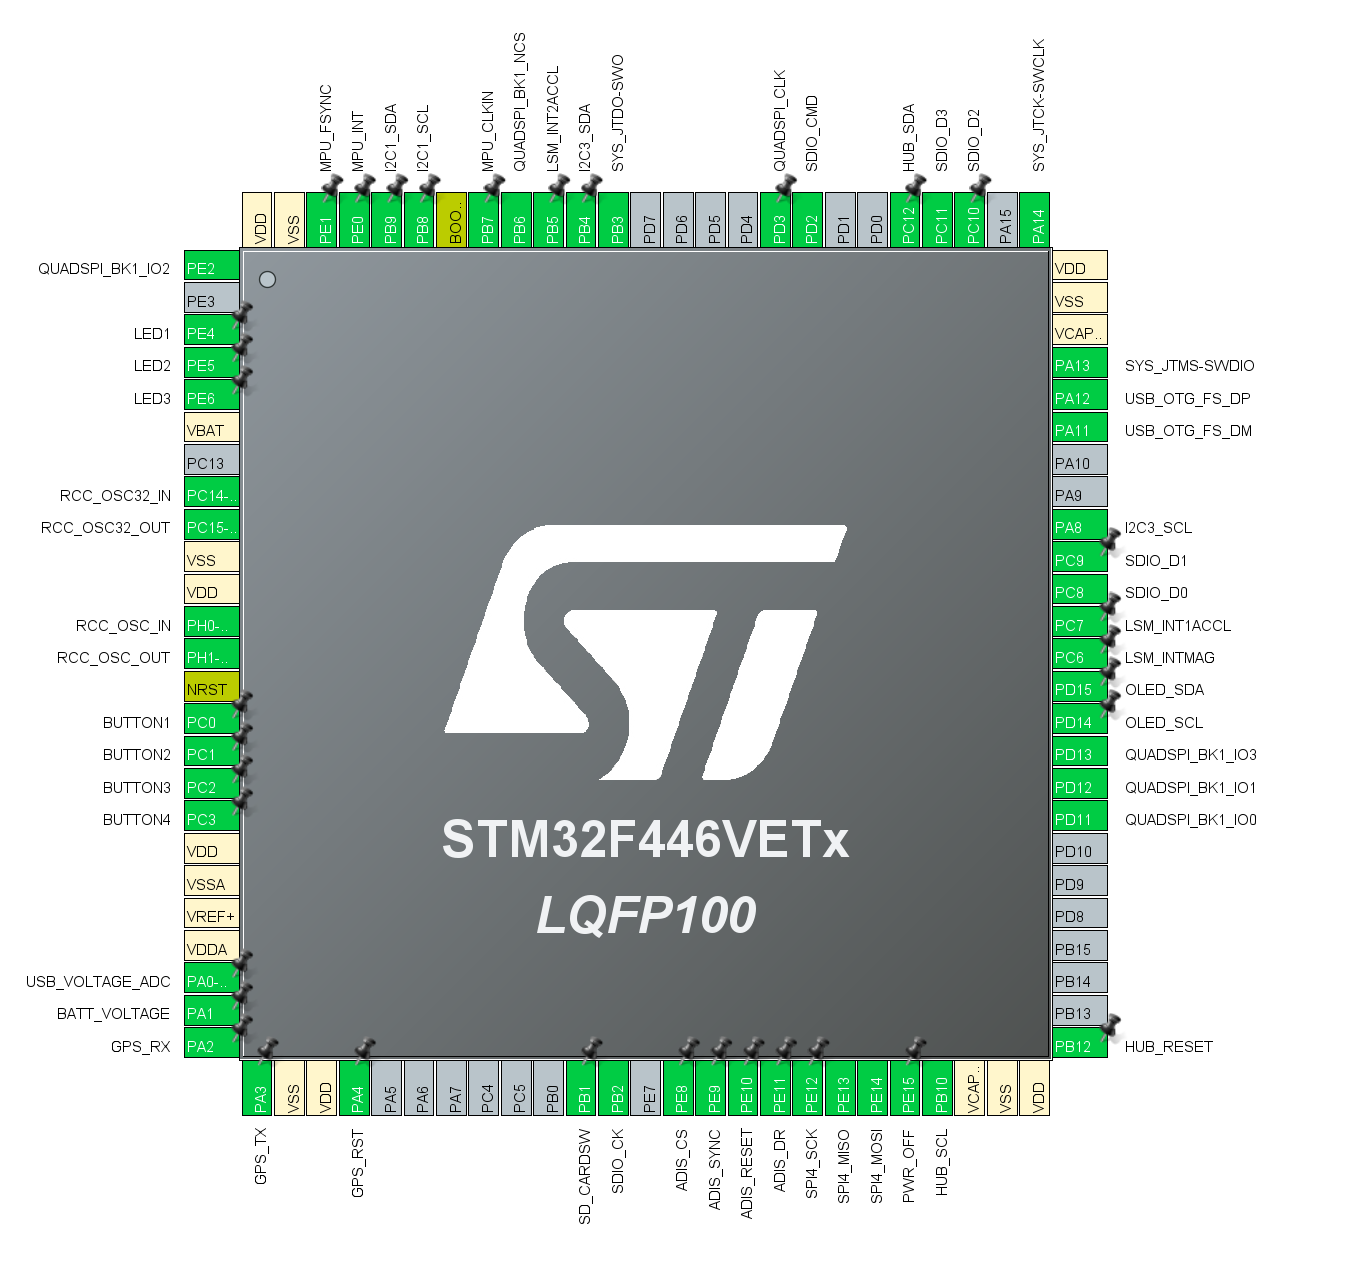
\includegraphics[width=\textwidth]{obrazky/cubePinout}
         \caption{Konfigurace pinů}
       
     \end{subfigure}
     \hfill
     \begin{subfigure}[b]{0.4\textwidth}
         \centering
         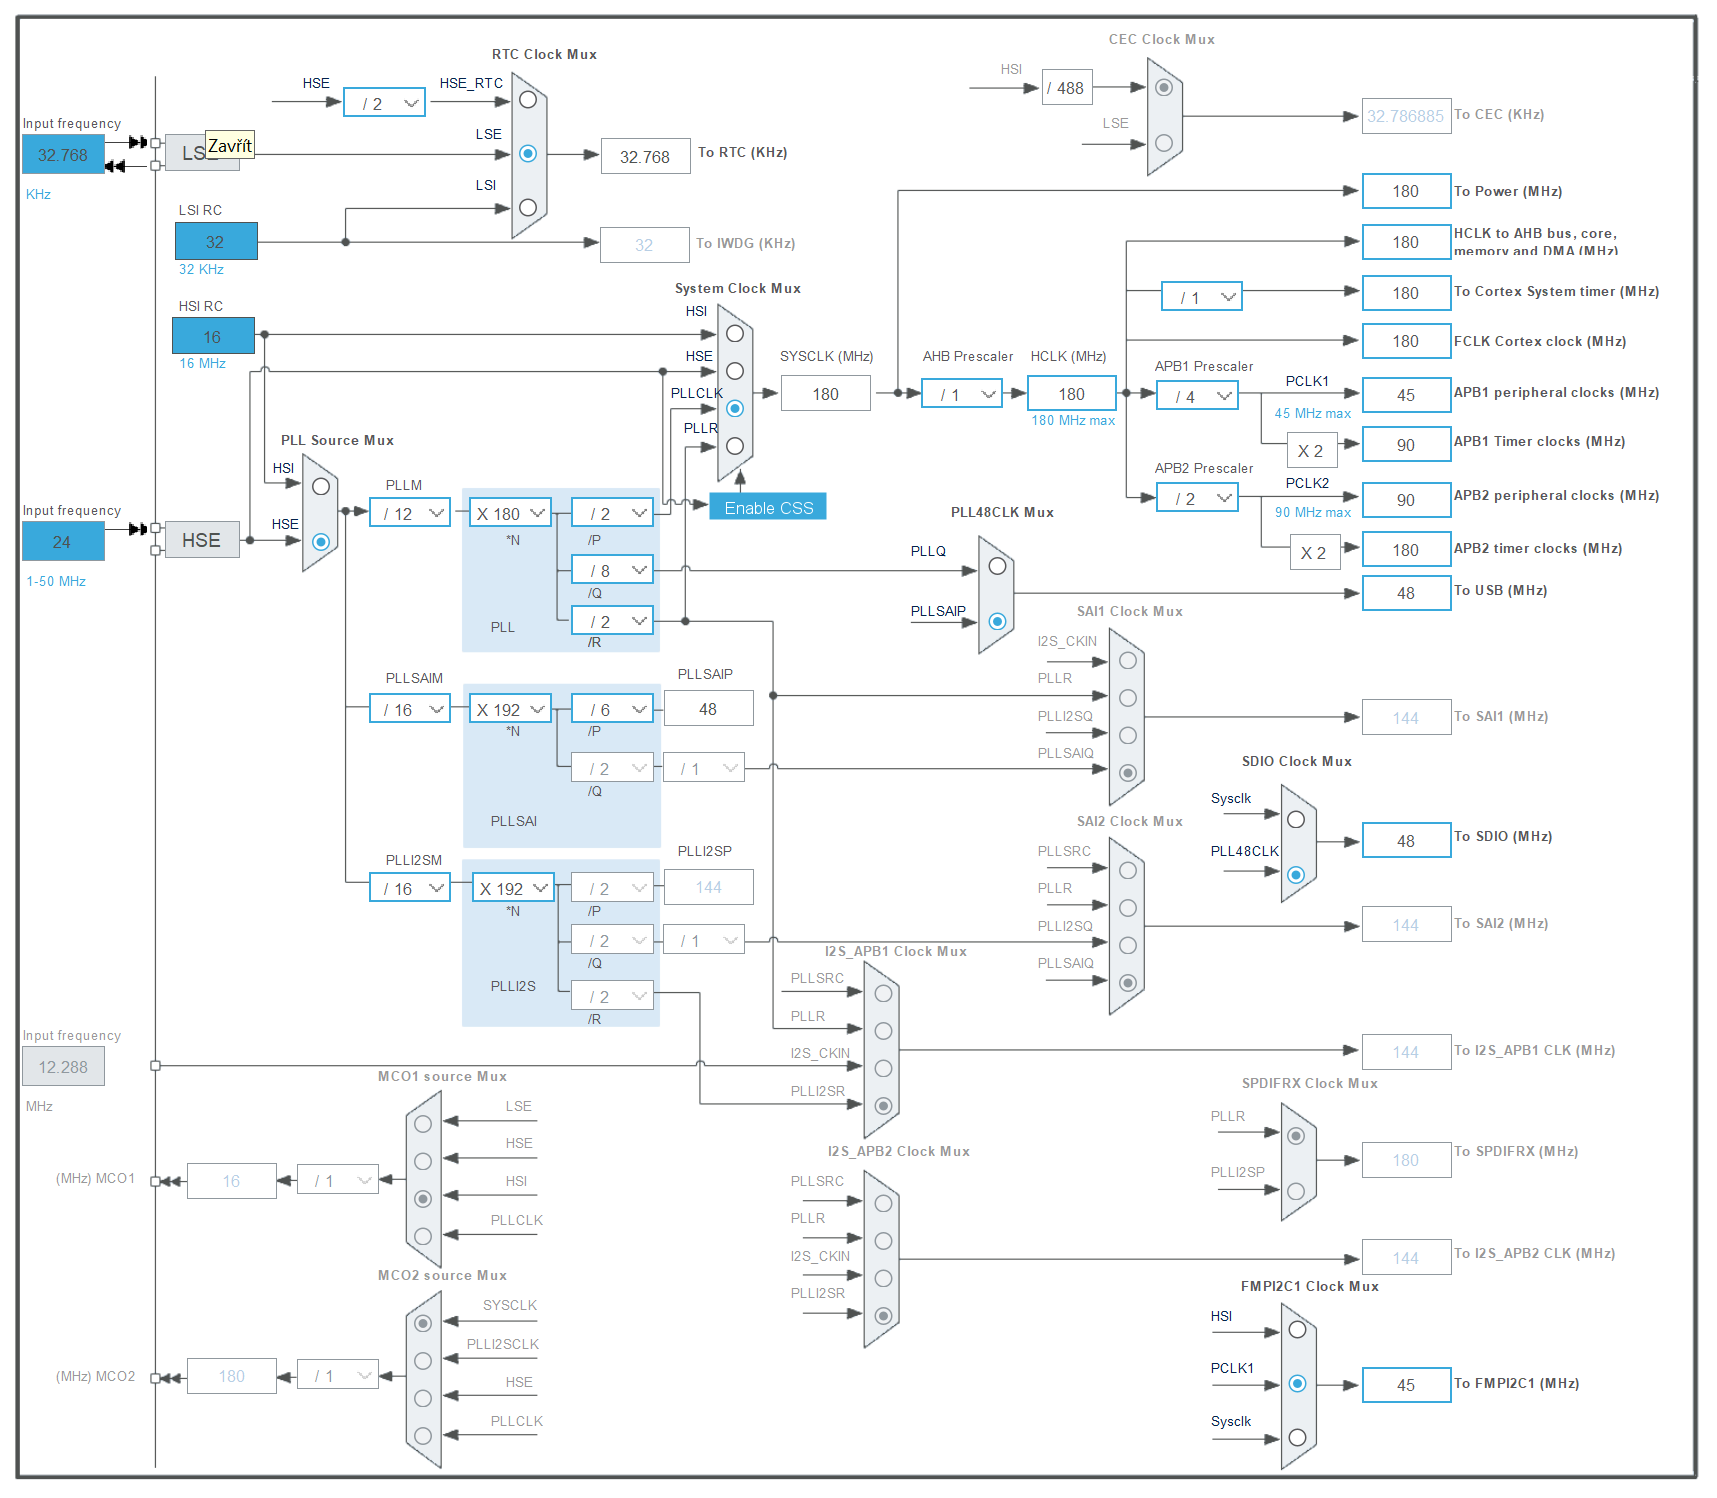
\includegraphics[width=\textwidth]{obrazky/cubeClock}
         \caption{Konfigurace hodin}
         
     \end{subfigure}
        \caption{Konfigurace MCU v STM32CubeIDE}
        \label{fig:cubeConfig}
\end{figure}

\section{FreeRTOS}
V této aplikaci je potřeba vyčítat, převádět a zapisovat data z několika různých senzorů které nemají přesně stejný hodinový signál, zároveň obsluhovat \ac{GUI} a provádět záznam dat zároveň. Pro potřeby synchronizace několika úloh, které nemají stejné periody, nebo například čekají na vstup od uživatele se hodí \ac{RTOS}.

Byla vybrána jedna z variant operačních systémů reálného času, a to FreeRTOS. Jedná se o jednoduchý open-source systém, který je hojně využíván ve vestavěných aplikacích. Umožňuje aplikaci virtuálně rozdělit na několik samostatných vláken (tzv. \emph{tasků}) s různými prioritami. Časování tasků je možné například pomocí neblokujících prodlev, nebo semaforů. FreeRTOS také plní funkci správy a alokace paměti. Předávání informací mezi jednotlivými tasky se provádí pomocí tzv. \emph{Queues}, díky tomu je možné se vyvarovat použití globálních proměnných. \cite{Zhu2011}

Práce s FreeRTOS je v STM32CubeIDE zjednodušená také díky poměrně dobré možnosti ladit aplikace pomocí již vestavěného RTOS-aware debuggeru, díky kterému můžeme například analyzovat využití paměti jednotlivých tasků, využití času, nebo kontrolovat stavy semaforů a velikost obsazených Queues. 

\section{Vývojové diagramy firmwaru}
Popsat chování a funkcionalitu firmwaru této aplikace dohromady by bylo poměrně nepřehledné. Proto budou jednotlivé funkce rozděleny do několika samostatných logických bloků, kde každý blok reprezentuje jeden task operačního systému.

\subsection{KeepaliveTask}
\begin{figure}[h]
    \centering
    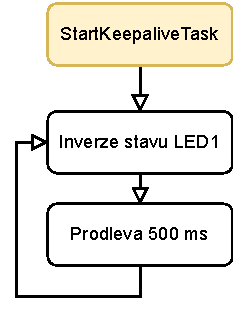
\includegraphics[width=0.3\textwidth]{obrazky/KeepaliveTask}
    \caption{Vývojový diagram KeepaliveTask}
\end{figure}
Jedná se o úlohu s nejnižší prioritou...

\subsection{hubTask}
\begin{figure}[h]
    \centering
    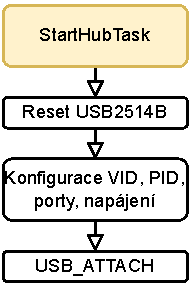
\includegraphics[width=0.3\textwidth]{obrazky/HubTask}
    \caption{Vývojový diagram HubTask}
\end{figure}
\subsection{powerTask}
\begin{figure}[h]
    \centering
    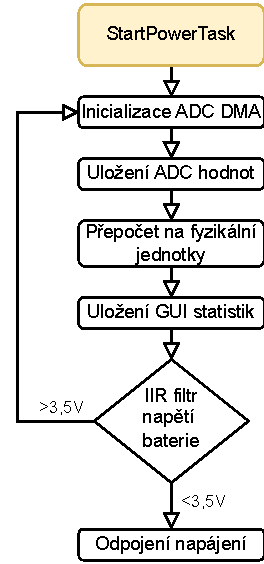
\includegraphics[width=0.3\textwidth]{obrazky/PowerTask}
    \caption{Vývojový diagram PowerTask}
\end{figure}
\subsection{gpsTask}
\begin{figure}[h]
    \centering
    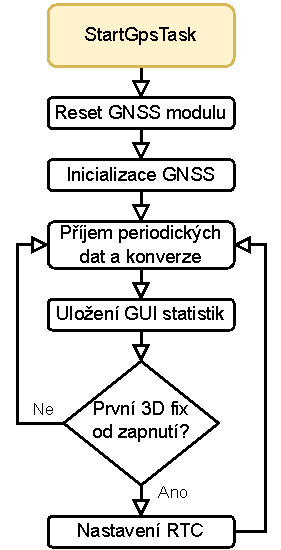
\includegraphics[width=0.3\textwidth]{obrazky/GpsTask}
    \caption{Vývojový diagram GpsTask}
\end{figure}
\subsection{lsmTask}
\begin{figure}[h]
    \centering
    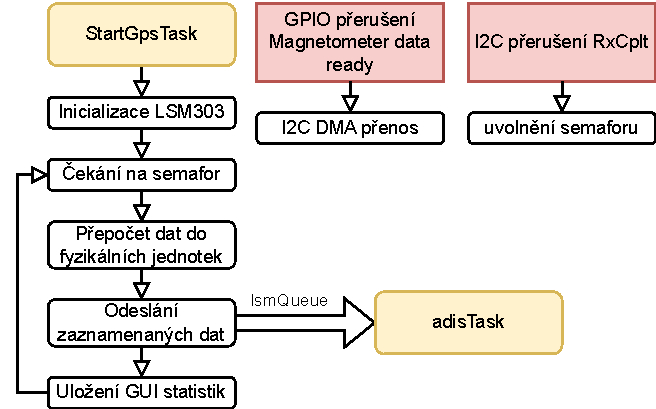
\includegraphics[width=0.6\textwidth]{obrazky/LsmTask}
    \caption{Vývojový diagram LsmTask}
\end{figure}
\subsection{mpuTask}
\begin{figure}[h]
    \centering
    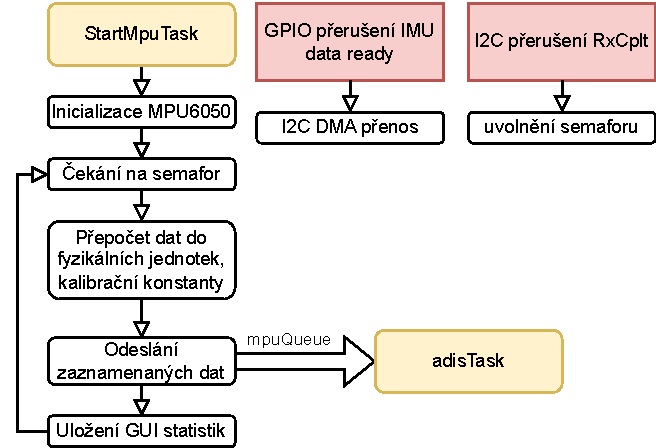
\includegraphics[width=0.6\textwidth]{obrazky/MpuTask}
    \caption{Vývojový diagram MpuTask}
\end{figure}
\subsection{adisTask}
\begin{figure}[h]
    \centering
    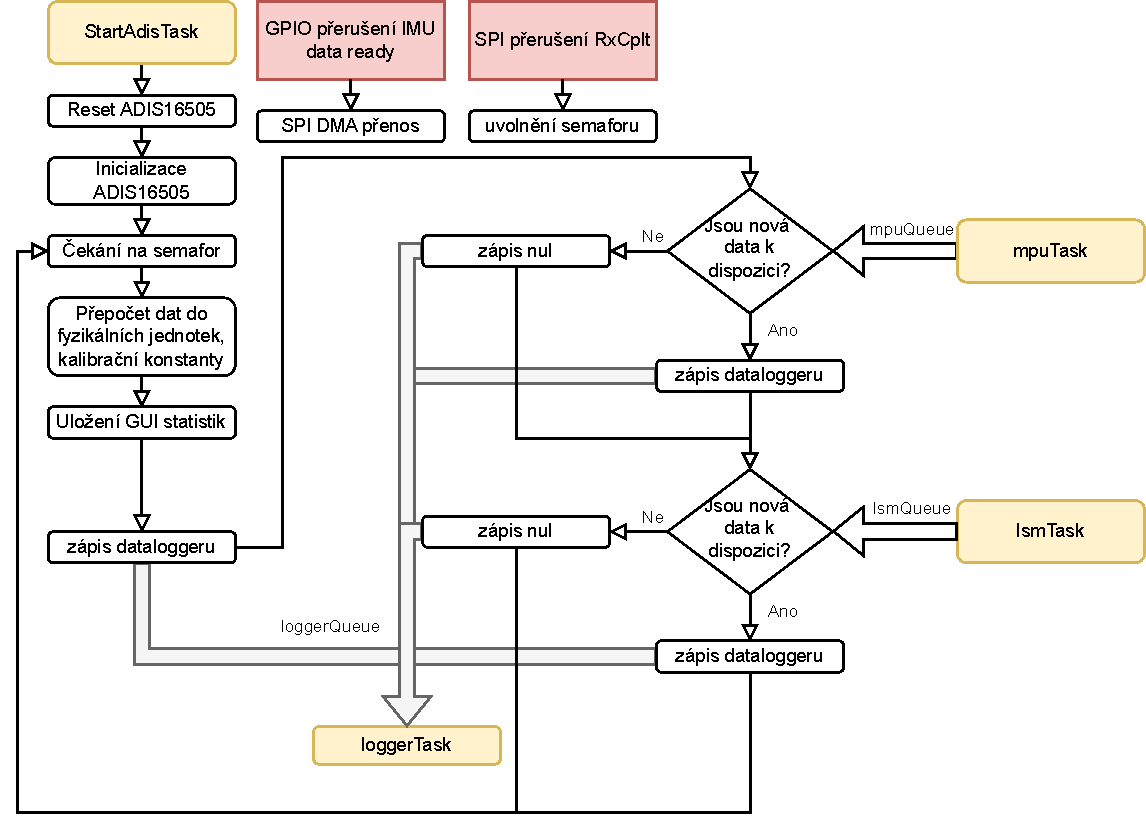
\includegraphics[width=0.95\textwidth]{obrazky/AdisTask}
    \caption{Vývojový diagram AdisTask}
\end{figure}
\subsection{loggerTask}
\subsection{oledTask}

...jednotlivé sekce a subsekce vývojových diagramů, hlavní vývojový diagram

gui

kalibrace

testy

zarovnávání bytů v paměti



